% !TeX root = ../tango.tex
\section{Background and Motivation}
\label{sec:background-and-motivation}

\subsection{Multi-SLO LLM Serving}
\label{sec:multi-slo-llm-serving}

\textbf{LLM Inference and Latency SLOs.}
An online LLM serving engine processes each request in two phases.
During \emph{prefill}, the engine processes all prompt tokens in parallel, constructs their key--value (KV) caches, and produces the first output token.
During \emph{decode}, it reuses the KV caches and autoregressively generates subsequent output tokens, typically one token per request in each iteration.
The two phases expose different forms of latency and corresponding service-level objectives (SLOs): a request must first wait for its prompt to be processed, and must then make timely progress over a sequence of decoding iterations.
Let request $r_i$ arrive at time $a_i$ and generate $n_i$ output tokens, where $t_{i,j}$ denotes the time at which its $j$-th output token is returned.
Its time to first token (TTFT) and time per output token (TPOT) are defined as
\begin{equation}
  \begin{aligned}
    \mathrm{TTFT}_i &= t_{i,1} - a_i, \\
    \mathrm{TPOT}_i &= \frac{1}{n_i-1}
      \sum_{j=2}^{n_i}\left(t_{i,j}-t_{i,j-1}\right),
      \quad n_i > 1.
  \end{aligned}
  \label{eq:latency-metrics}
\end{equation}
TTFT captures the queuing and prefill delay before a response begins, whereas TPOT captures the average interval between consecutive tokens after generation starts.
Each request is associated with a pair of latency objectives, denoted by $S_i^{\mathrm{TTFT}}$ and $S_i^{\mathrm{TPOT}}$.
Request $r_i$ satisfies its SLOs only if
$\mathrm{TTFT}_i \leq S_i^{\mathrm{TTFT}}$ and
$\mathrm{TPOT}_i \leq S_i^{\mathrm{TPOT}}$.
In this work, \emph{Multi-SLO} refers both to these phase-specific objectives and to their heterogeneous values across requests and applications.
Accordingly, serving efficiency is measured by goodput---the rate of requests that satisfy both objectives---rather than by raw request or token throughput alone.

\textbf{Continuous Batching and Chunked Prefill.}
In static batching, a newly arrived request cannot join an executing batch until every request in that batch finishes, which wastes GPU capacity as requests complete at different times.
Continuous batching instead updates the active batch at iteration boundaries.
After each iteration, completed requests leave, unfinished decode requests remain active, and waiting requests can be admitted into the released capacity.
The batch composition can thus evolve throughout generation, improving GPU utilization while allowing the scheduler to reconsider which requests should run at every step.

A prefill request may contain hundreds or thousands of prompt tokens, whereas an active decode request contributes only its next token to an iteration.
Scheduling an entire prompt at once can therefore produce a long iteration and delay token generation for the decode requests in the same batch.
Chunked prefill divides the prompt into smaller chunks that may be processed over multiple iterations.
This enables prefill chunks and decode tokens to be colocated in one batch, while exposing the prefill chunk size as a controllable scheduling variable.
Specifically, let $\mathcal{P}_k$ and $\mathcal{D}_k$ denote the prefill and decode requests selected in step $k$, respectively, and let $c_{i,k}$ be the number of prompt tokens allocated to prefill request $r_i$.
The number of tokens scheduled in this step is
\begin{equation}
  T_k = \sum_{r_i \in \mathcal{P}_k} c_{i,k}
        + \lvert\mathcal{D}_k\rvert,
  \qquad T_k \leq B_{\max},
  \label{eq:step-token-budget}
\end{equation}
where each decode request contributes one token and $B_{\max}$ is the engine's maximum per-step token budget.
The resulting queueing delay and intervals between decoding iterations determine whether each request meets its TTFT and TPOT objectives.

\subsection{Multi-SLO Traces for Investigations}
\label{subsec:motivation-trace}

We construct three representative LLM inference workloads covering conversational assistance, mathematical reasoning, and software-engineering agents.

\textbf{Chatbots.}
We construct chatbot requests from LMSYS-Chat-1M, which contains one million real-world conversations collected from interactions with 25 LLMs.
The token length of each recorded response determines its target output length.

\textbf{Mathematical Reasoning.}
We use all 8,792 questions from the training and test splits of GSM8K.
Each word problem serves as the input prompt, while the token length of its reference solution determines the target output length.

\textbf{Software Agents.}
We use the software-engineering subset of AgentWorldBench and retain one request from each of 99 distinct trajectories.
For each request, we generate 1,024 variants by prepending a distinct synthetic prefix while preserving the original agent action and target environment observation.

From the three request pools, we randomly sample 10,000 chatbot, 8,000 mathematical-reasoning, and 4,000 software-agent requests to form the replay traces.


\textbf{Arrivals and SLOs.}
We associate requests in order with timestamps from failure-free entries in BurstGPT and replay each workload according to these timestamps, thereby preserving the trace's temporal arrival pattern.
For each workload, we first determine the sending rate $\lambda_{90}$ at which vLLM achieves a 90\% SLO attainment rate.
We then set the sending rate to $1.2\lambda_{90}$ to emulate a workload under pressure.

For each request, we execute it alone on an otherwise idle vLLM deployment and record its measured TTFT and TPOT.
These isolated measurements serve as request-specific latency baselines.
We derive the two SLOs of request $r_i$ as
\begin{equation}
  \begin{aligned}
    S_i^{\mathrm{TTFT}} &= c_i^{\mathrm{TTFT}}
      \widehat{\mathrm{TTFT}}_i, \\
    S_i^{\mathrm{TPOT}} &= c_i^{\mathrm{TPOT}}
      \widehat{\mathrm{TPOT}}_i,
  \end{aligned}
  \label{eq:slo-generation}
\end{equation}
where $\widehat{\mathrm{TTFT}}_i$ and $\widehat{\mathrm{TPOT}}_i$ are the isolated-run measurements, and $c_i^{\mathrm{TTFT}}$ and $c_i^{\mathrm{TPOT}}$ are the coefficients assigned to the request's SLO class.
Using a fixed random seed, we assign requests equally among four SLO classes: TTFT-prioritized, TPOT-prioritized, balanced, and relaxed.
For Qwen3-14B, the TTFT/TPOT coefficient pairs for these four classes are $(20, 2.5)$, $(50, 1.5)$, $(25, 2)$, and $(50, 3)$, respectively.
All compared systems use the same request sequence, arrival schedule, and SLO targets under each experimental condition.



\begin{table}[t]
  \renewcommand{\arraystretch}{1.05}
  \setlength{\tabcolsep}{3pt}
  \caption{Experimental setup.}
  \label{tab:motivation-setup}
  \centering
  \scriptsize
  \resizebox{\columnwidth}{!}{%
  \begin{tabular}{c|c}
    \hline
    & \textbf{Specifications} \\
    \hline
    \textbf{Hardware} & \makecell[c]{$2\times$ Intel Xeon Gold 6530 CPUs, 64 physical cores \\
      128 logical threads, 377.6 GiB host RAM (OS-reported) \\
      $4\times$ RTX 6000 Ada GPUs (48 GB each); $2\times$ GPUs used per run} \\
    \hline
    \textbf{Software} & \makecell[c]{Qwen/Qwen3-14B (TP${}={}$2); vLLM 0.17.0 \\
      PyTorch 2.10.0+cu128; CUDA 12.8; driver 570.124.06 \\
      LMSYS-Chat-1M, GSM8K, AgentWorldBench-SWE, BurstGPT} \\
    \hline
  \end{tabular}%
  }
\end{table}

\subsection{Low Multi-SLO Serving Performance}
\label{subsec:low-multi-slo-performance}

\begin{table}[t]
  \centering
  \caption{SLO attainment of vLLM on the math workload.}
  \label{tab:fcfs-multi-slo-attainment}
  \scriptsize
  \setlength{\tabcolsep}{3pt}
  \renewcommand{\arraystretch}{1.10}
  \begin{tabular}{lccc}
    \hline
    \textbf{SLO Class} &
    \textbf{TTFT (\%)} &
    \textbf{TPOT (\%)} &
    \textbf{Joint (\%)} \\
    \hline
    Overall          & \textbf{75.80} & \textbf{77.68} & \textbf{53.48} \\
    TTFT-prioritized & 48.89 & 100.00 & 48.89 \\
    TPOT-prioritized & 100.00 & 12.00 & 12.00 \\
    Balanced         & 57.39 & 100.00 & 57.39 \\
    Relaxed          & 100.00 & 100.00 & 100.00 \\
    \hline
  \end{tabular}
\end{table}

We use vLLM's default FCFS scheduler as a representative serving baseline.
It supports continuous batching and chunked prefill, but schedules requests without differentiating their TTFT and TPOT objectives.
We run Qwen3-14B with TP${}={}$2 on two GPUs using the configuration in Table~\ref{tab:motivation-setup}.
We use the math workload as a representative case and replay it at its stress load of $1.2\lambda_{90}$.

Table~\ref{tab:fcfs-multi-slo-attainment} summarizes the SLO attainment rates for the math workload.
Under FCFS, the overall TTFT and TPOT attainment rates are 75.80\% and 77.68\%, respectively, but only 53.48\% of requests satisfy both objectives.
The gap between individual and joint attainment shows that satisfying either latency objective alone does not provide effective Multi-SLO service.

The class-level results further reveal distinct failure modes.
TTFT-prioritized requests achieve 48.89\% TTFT attainment and 100.00\% TPOT attainment, whereas TPOT-prioritized requests achieve 100.00\% and 12.00\%, respectively.
Balanced and relaxed requests attain both objectives for 57.39\% and 100.00\% of their requests, respectively.
The contrasting class-level results indicate that the low joint attainment cannot be attributed to a single global latency bottleneck.

Together, these observations expose a mismatch between throughput-oriented scheduling and request-specific latency objectives.
FCFS fixes the service order according to request arrival and does not account for the remaining TTFT or TPOT slack when admitting prefill chunks or advancing decode requests.
Consequently, a scheduling decision that preserves prompt responsiveness may disrupt token delivery, while one that protects decode progress may increase the waiting time of queued prefills.
The serving engine can therefore retain sufficient capacity to satisfy 100.00\% of the relaxed requests, yet fail to direct that capacity toward the phase-specific objectives of other requests.
These observations motivate a closer examination of how request ordering and per-step token allocation jointly affect Multi-SLO attainment.

\subsection{Diving into Underlying Reasons}
\label{subsec:motivation-underlying-reasons}

Our investigation identifies two complementary causes of the low Multi-SLO attainment: 1) FCFS distributes queueing delay without considering request-specific TTFT urgency, and 2) a fixed token budget does not provide a reliable latency bound for steps that mix prefill and decode tokens.

\begin{figure}[!t]
  \centering
  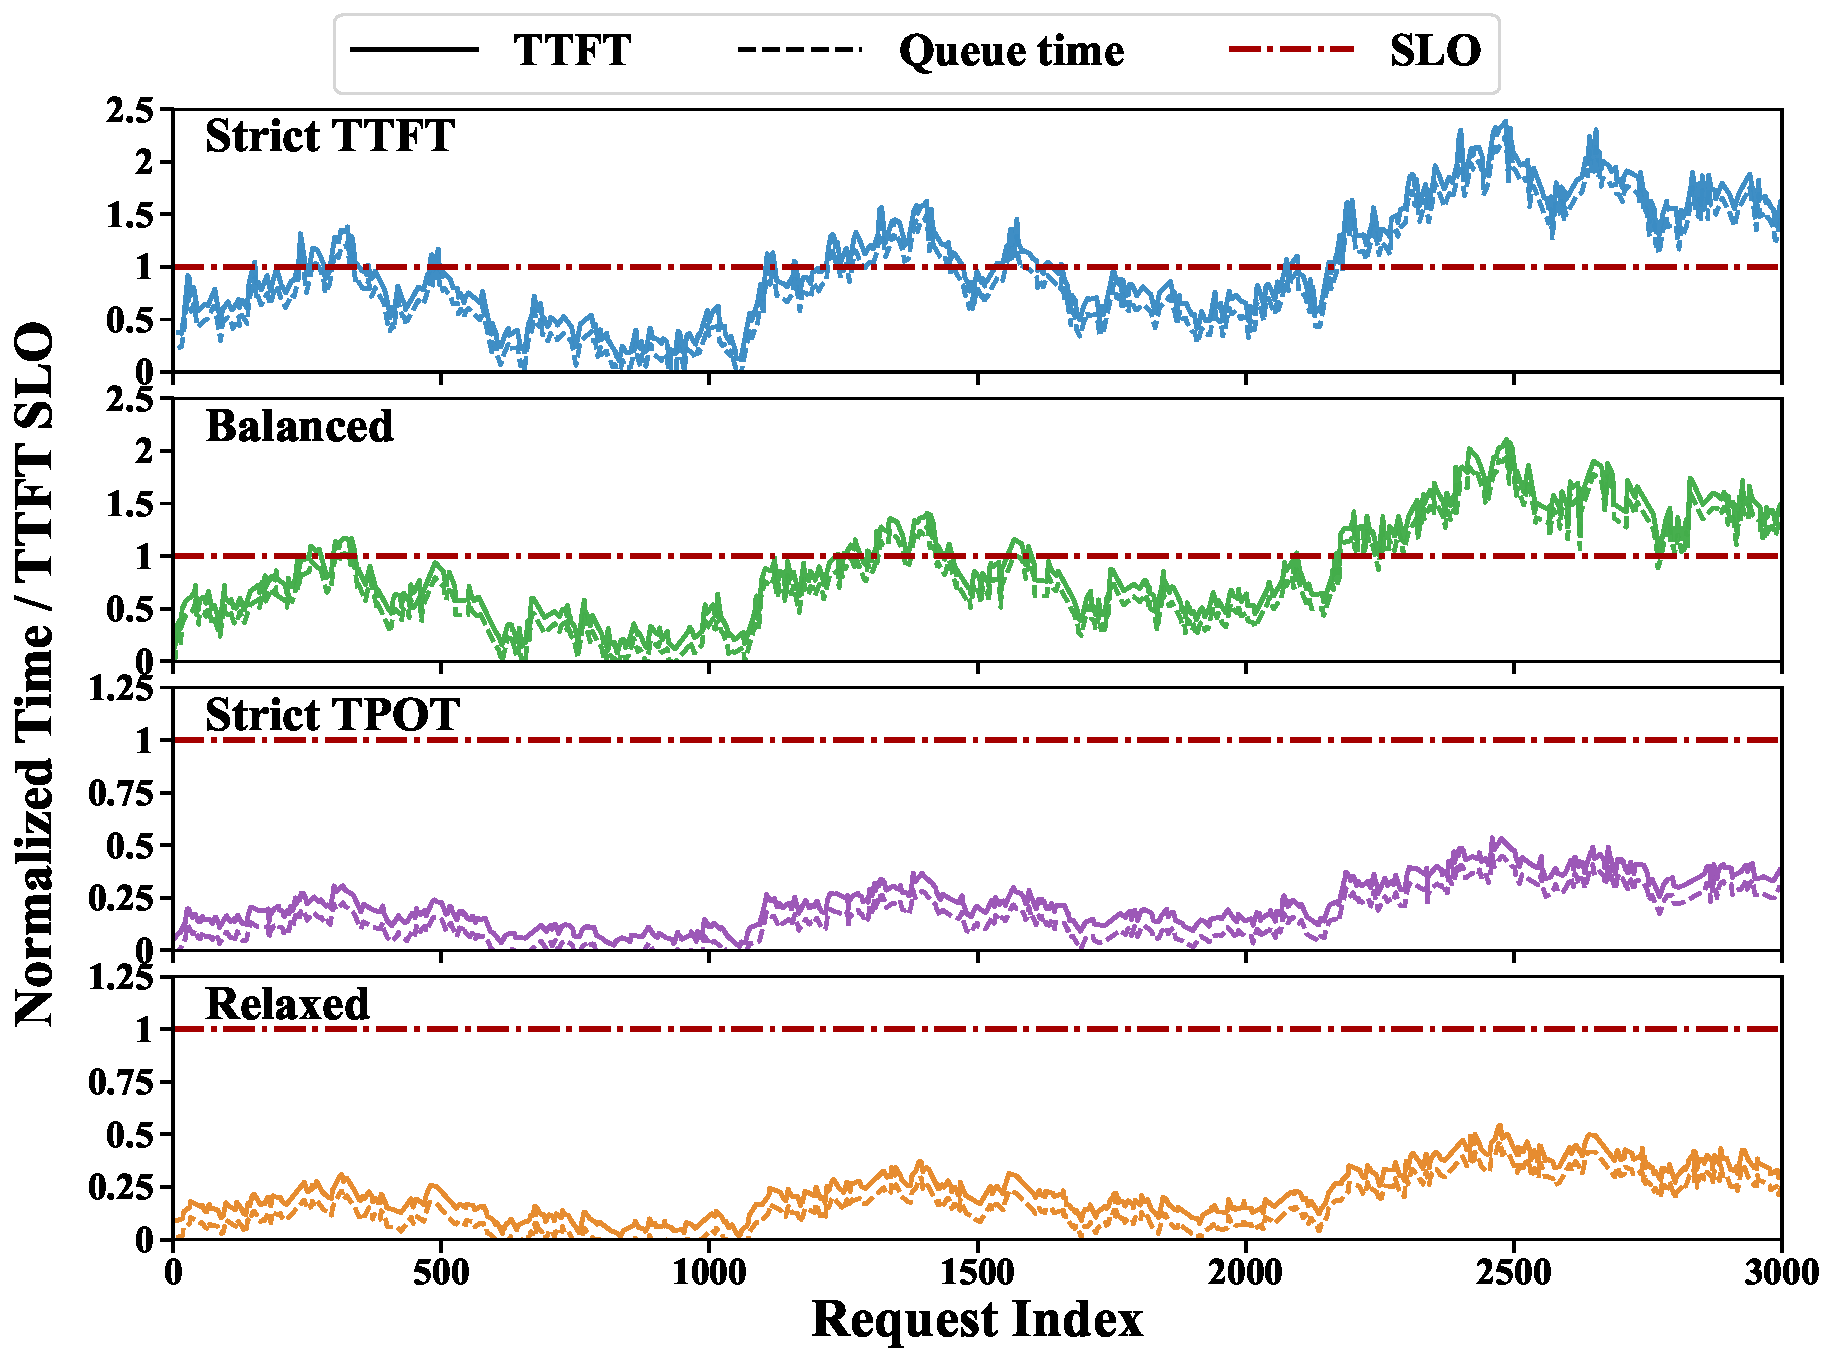
\includegraphics[width=0.94\columnwidth]{figures/background-and-motivation/moti_queue_slo}
  \caption{Normalized TTFT and queueing time under FCFS.}
  \label{fig:temporal-slo-ratio}
\end{figure}

\noindent\textbf{1) SLO-unaware temporal scheduling.}
The first-token latency of request $r_i$ can be decomposed as
\begin{equation}
  \mathrm{TTFT}_i = W_i^{\mathrm{queue}} + L_i^{\mathrm{prefill}},
  \label{eq:ttft-decomposition}
\end{equation}
where $W_i^{\mathrm{queue}}$ is the delay from arrival until the request is first admitted for prefill, and $L_i^{\mathrm{prefill}}$ is the remaining latency until its first token is produced.
For a chunked prefill, $L_i^{\mathrm{prefill}}$ includes the execution and intervening scheduling delays of all prompt chunks after admission.

Fig.~\ref{fig:temporal-slo-ratio} plots TTFT and queueing time for the first 3,001 math requests, normalized by each request's TTFT SLO.
Solid and dashed lines denote TTFT and queueing time, respectively; the dash-dotted line marks the SLO boundary.
The Strict TTFT and Strict TPOT panels correspond to the TTFT-prioritized and TPOT-prioritized classes, respectively.
The normalized queueing-time curve closely follows the TTFT curve in all four SLO classes, indicating that queueing dominates the first-token latency.
For TTFT-prioritized and balanced requests, the queueing delay frequently consumes most, or even all, of the TTFT budget before prefill completes.
TPOT-prioritized and relaxed requests remain below the boundary because their looser TTFT objectives provide substantially more slack.
The resulting TTFT violations therefore arise primarily from how waiting time is distributed among requests, rather than from a uniform shortage of prefill compute capacity.

FCFS creates this imbalance because it admits requests according to arrival order, regardless of their remaining TTFT slack.
A TTFT-prioritized request may wait behind earlier requests whose looser objectives could tolerate additional delay; the urgent request exhausts its latency budget in the queue while those ahead of it still finish within their SLOs.
The temporal scheduling problem is thus to determine \emph{which request} should receive prefill service first.
Accounting for the remaining TTFT slack can redistribute queueing delay toward requests that can tolerate it, without changing the total amount of prefill work.

\begin{figure}[!t]
  \centering
  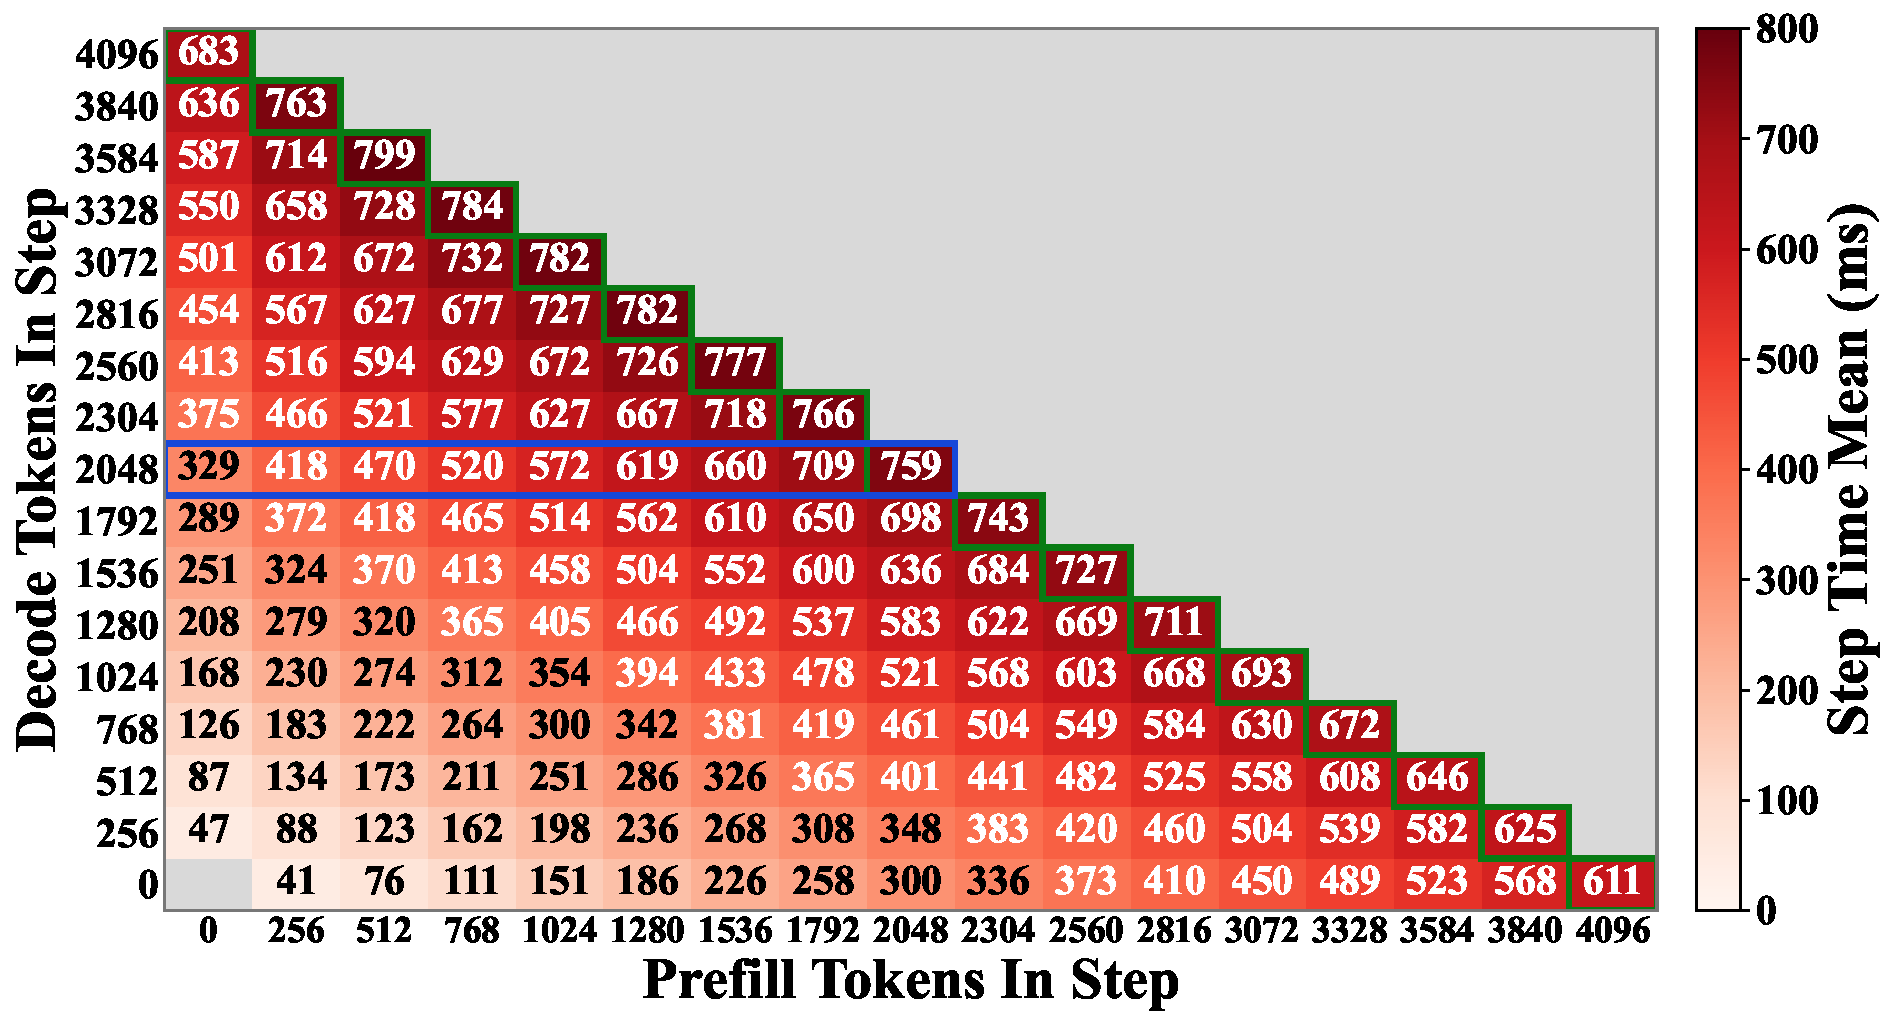
\includegraphics[width=\columnwidth]{figures/background-and-motivation/moti_token_heatmap}
  \caption{Mean step time with different prefill and decode token counts.}
  \label{fig:spatial-pd-grid}
\end{figure}

\noindent\textbf{2) Workload-unaware spatial scheduling.}
The second failure mode arises after requests enter the running batch.
For an active decode request, the interval before its next token is determined by the duration of the engine step in which that token is scheduled.
Reordering waiting requests alone cannot protect TPOT because a decode token may still share a step with a large prefill chunk.

To quantify this interference, we vary the numbers of prefill tokens $p$ and decode tokens $d$ scheduled in the same step and measure the mean step time.
Each configuration is measured on Qwen3-14B with TP${}={}$2 over 50 timed steps (5 rounds $\times$ 10 measurements); gray cells exceed the maximum per-step token budget.
As highlighted by the blue outline in Fig.~\ref{fig:spatial-pd-grid}, when $d=2{,}048$, increasing $p$ from 0 to 2,048 increases the mean step time from 329\,ms to 759\,ms.
Every active decode request must wait for the longer step to complete before receiving its next token, directly increasing its TPOT.

More importantly, the total token count alone does not determine step time.
Along the green boundary where $p+d=4{,}096$, the pure-prefill and pure-decode configurations take 611\,ms and 683\,ms, respectively, while mixed configurations reach up to 799\,ms.
Thus, the same total token budget produces about a $1.3\times$ difference in latency.
This nonlinearity reflects the distinct execution characteristics of compute-intensive prefill and memory-intensive decode, together with their interference when colocated in one iteration.
Consequently, enforcing only $p+d\leq B_{\max}$ bounds the amount of scheduled work but cannot reliably bound the wall-clock latency experienced by active decode requests.

The spatial scheduling problem is therefore to determine \emph{how many prefill tokens} can safely share the next step with the current decode workload.
This requires an estimate of mixed-step latency and a mechanism that converts the remaining TPOT slack of active requests into a safe prefill allocation.
Temporal request ordering and spatial token allocation address different failure modes: optimizing either dimension alone leaves the other source of SLO violations unresolved.
These observations motivate their joint design in \tango{}.
